\section{Overview of the approach}
\label{sec:overview}
Fig.~\ref{fig:underlying} describes the underlying process we aim to model:
given a discrete feature map $I[i,j]$, we are interested in constructing \niv{a} CC-layer that operates on $I$ as an input, and produces a next layer $I'[i',j']$, by modeling a learned continuous convolution between the input and output feature-maps.
%$I$ and $I'$. 
Note that the input and output feature-maps  $I$ and $I'$ need \emph{not} be related by an integer  scale factor (or its inverse).
%
Such \niv{an} action can be realized by \niv{the following steps}: 
\vspace*{0.1cm} \\ 
(i)~Use a ''Bed of Nails'' representation of $I$:
$I_{cont}(h,w) = \sum_{i,j}\delta(h-i, w-j)I[i,j]$.
where $i,j$ are discrete `pixel' (feature) locations in $I$, and $h,w$ are continuous coordinates in the continuous feature-map space. 
%For simplicity, we will refer from here on  to all discrete coordinates inside feature maps \niv{(whether input images or the outputs of intermediate network layers)} by the term \textbf{`pixels'}, and their in-between non-integer coordinates as \textbf{sub-`pixel'}. 
For simplicity, {we will refer from here on  to all discrete coordinates inside feature maps by the term \textbf{`pixels'}, and their in-between non-integer coordinates as \textbf{sub-`pixel'} (although we are referring to general network layers; usually not images)}. 
\vspace*{0.1cm} \\
(ii)~Apply a convolution with a \emph{learned} continuous kernel $\mathcal{K}_\theta(h,w)$.
\vspace*{0.1cm} \\
(iii)~Resample the continuous result of the convolution according to the desired shape and scale-factors of $I'$. The resampling grid is purely a function of the shape and scales.
%and the only function of them in the process. 
This means that the same continuous kernel $\mathcal{K}_\theta$ is eligible for producing any desired scale-factor for $I'$.

These phases are indicated in Fig.~\ref{fig:underlying}, and can be mathematically formulated as follows:
\begin{align}
    CC\{I\}[\textbf{n}] = \{I_{cont} * \mathcal{K}_{\theta}\}(\textbf{g}_n)
    &=
   \iint\sum_{\textbf{m}}\delta
   \left(\textbf{g}_n-\mathbf{\tau}-\textbf{m}\right)
    I[\textbf{m}] \mathcal{K}_\theta(\mathbf{\tau})d \mathbf{\tau} \notag\\
    &=
  \sum_{\textbf{m}}I[\textbf{m}]\iint
  \Big(\delta\left(
  \textbf{g}_n-\mathbf{\tau}-\textbf{m}\right)
     \mathcal{K}_\theta(\mathbf{\tau})\Big)d \mathbf{\tau} \notag\\
    % \iintertext{The Dirac Delta function implies that a non-zero contribution only occurs when $\mathbf{\tau}=\textbf{g}_n-\textbf{m}$.} 
   &=\sum_{\textbf{m}}
     I[\textbf{m}]\mathcal{K}_\theta(\textbf{g}_n-\textbf{m})
\label{eq:underlying}
\end{align}



% \niv{alternative for next \underline{two} paragraphs: 
where $\textbf{m}=(i,j),  \textbf{n}=(i',j')$ are discrete `pixel' coordinates in $I$ and $I'$ respectively, and $\textbf{g}_n$ denotes the continuous sampling locations of the grid
in Fig.~\ref{fig:underlying} 
(i.e., the sub-`pixel' position of  each `pixel' in $I'$ when projected onto the coordinates of $I$). 

Eq.~\ref{eq:underlying} shows that for $\mathcal{K}_\theta$ with finite support, the output of the continuous convolution at $I'[\textbf{n}]$ is a weighted sum of the discrete ``Neighbors'' of its projected location  $\textbf{g}_n$ in the input $I$. The weights are a function of the distance between the discrete `pixel' center  $\textbf{m}$  to the continuous sampling location~$\textbf{g}_n$.
%
The desired sampling grid \varbold{$\textbf{g}_n$} is calculated by projecting the output integer `pixel' locations $\textbf{n}=(i',j')$ in $I'$, to sub-`pixel' coordinates in the input $I$. 
We call it the {``Projected Grid''}. 

% Assuming \niv{If?} $\mathcal{K}_\theta$ has finite support, there is a constant number of set of indices $\textbf{m} \in I$ that contribute to $\textbf{n}$ \niv{we've already mentioned it above, though non-rigorously as in here. but better just drop one of them, otherwise it's redundant}. 
% We call these the \textbf{Neighbors} of the projected grid point $\textbf{g}_n$, and denote them by $\varbold{\mathcal{N}\textbf{[n]}}$. Each such set of neighbors has a corresponding 
% set of  learnable \textbf{Weights};
% $\varbold{\mathcal{W}\textbf{}{[n,m]}} = \mathcal{K}_\theta(\textbf{g}_n-\textbf{m})$.
% Once these three tensors are extracted, Eq.~\ref{eq:underlying} can be modeled.


% where $\textbf{n},\textbf{m}$, $\textbf{g}_n$ denote 2D vectors:   $\textbf{m}=(i,j),  \textbf{n}=(i',j')$ are the discrete `pixel'  coordinates in $I$ and $I'$ respectively, and $\textbf{g}_n$ denotes the continuous sampling locations of the grid in Fig.~\ref{fig:underlying} 
%(i.e., the sub-`pixel' position of  each `pixel' $(i',j')\in I'$ \niv{consider removing $(i',j')\\$ as these are coordinates, and also it's enough to just say "in I"} when projected onto the coordinates  of layer $I$).

% Eq.~\ref{eq:underlying} shows that the learned continuous convolution values \niv{maybe "outputs" instead of "values", as it's not clear. readers might confuse values to be either the outputs or the set of weights} are obtained from discrete feature values at `pixel' centers $I[\textbf{m}]$, multiplied by weights which 
% are a function of the distance between the discrete `pixel' center  $\textbf{m}$  to the continuous sampling location $\textbf{g}_n$. 
% In other words, if $\mathcal{K}_\theta$ has a finite support, every output neuron is a weighted sum of the discrete ``neighbors'' of its projected location in the input layer. 


% \section{Method}
\begin{figure}[t]
\vspace*{-1cm}
    \centering
%    \hspace*{-0.5in}
%    \includegraphics[width=1.3\textwidth]{figs/fig_overview.jpg}
    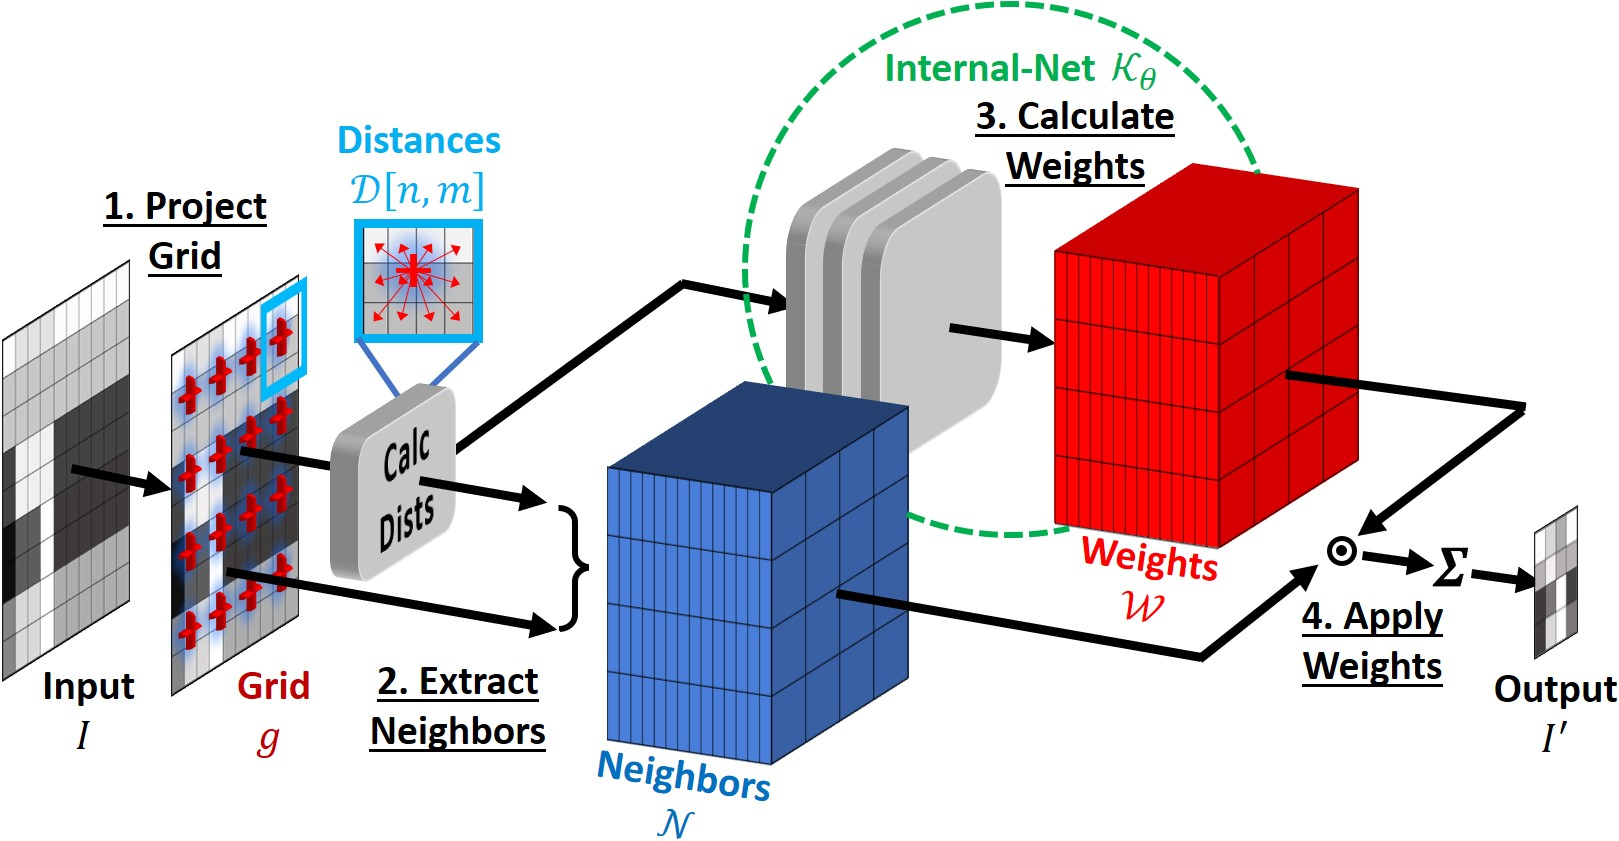
\includegraphics[width=0.9\textwidth]{figs/fig_overview_Ben.jpg}
    \caption{\it Overview of CC-layer. \ (see Sections~\ref{sec:overview} and~\ref{sec:implement} for details)}
    \label{fig:overview}
    \vspace*{-0.3cm}
\end{figure}

%\textbf{CC Overview:} 
% In order to execute our approach we need to overcome an inherent challenge:
% CNNs are built upon regular grids with discrete coordinates. We need to model a continuous process with discrete components. 
%Moreover, the final model needs to be end-to-end trainable by back propagation. \niv{next sentence is redundant} Our proposed construction of the CC-layer extracts all the components of Eq.~\ref{eq:underlying} and executes them.


In order to execute our approach we need to overcome an inherent challenge:
CNNs are built upon regular grids with discrete coordinates. 
We therefore need to model a continuous process with discrete components. 
Fig.~\ref{fig:overview} illustrates our CC-layer construction, which builds upon implementation ideas from standard image resizing techniques~\cite{MATLAB:2010}. 
Our CC-layer consists of 4 principled building blocks. These are marked by numbers in Fig.~\ref{fig:overview}, and are described in detail in Sec.~\ref{sec:implement}: 
\begin{enumerate}[noitemsep,nolistsep,leftmargin=*]
% \item \textbf{Calculate Projected Grid \varbold{$\textbf{g}_n$}:} 
% The desired sampling grid \varbold{$\textbf{g}_n$} is calculated by projecting the output integer `pixel' locations $\textbf{n}=(i',j')$ in $I'$, to sub-`pixel' coordinates in the input $I$. 
%We call it the \textbf{Projected Grid}. 
\item \textbf{Calculate Projected Grid \varbold{$\textbf{g}_n$}} 
from the desired scale-factors and  output-shape. 
% This is done both at train and at test time.
\item \textbf{Extract Neighbors \varbold{${\mathcal{N}}$}:} Map each sampling point $\textbf{g}_n$ to its discrete neighbors \varbold{${\mathcal{N}}[\textbf{n}]$} within the continuous kernel support. 
% This is done both at train and at test time.
\item \textbf{Calculate Weights} \varbold{$\mathcal{W}$} by applying \textbf{$\mathcal{K}_\theta$} to distances between sampling points to their neighbors:
$\varbold{\mathcal{W}\textbf{}{[n,m]}} = \mathcal{K}_\theta(\textbf{g}_n-\textbf{m})$.
%This is the only learnable part (learned at train-time). 
This ``Internal-Net''  \textbf{$\mathcal{K}_\theta$} is the only trainable part in the CC-layer.
%also the only part of the CC-layer that is kept in memory during train and test time. 
%\textbf{\textcolor{red}{Please circle Internal-Net in Fig2 by a green dashed line and add in green: \textcolor{cyan}{Internal-Net  \textbf{$\mathcal{K}_\theta$}}}}
\item \textbf{Apply Weights:}  Multiply \varbold{$\mathcal{N} \odot \mathcal{W}$} and sum over all neighbors and input channels, to obtain the output \ben{feature map} $I'$, with any desired scale or shape (which can be determined at test time).
\end{enumerate}

% Sec.~\ref{sec:implement}  describes in detail each of these four CC blocks, and explains how to train the dynamic CC-layer to allow for dynamic scale-generalization at test time. Sec.~\ref{sec:features} reviews the properties and benefits of the CC-layer, and presents new approaches for \emph{dynamic architectural design}, which become possible with the new CC-layer.  In Sec.~\ref{sec:efficiency} we specify ways to efficiently train CC. Finally, Sec.~\ref{sec:applications}  showcases a few possible ways to exploit CC-layers in various Computer Vision tasks. 
% \assaf{I would drop this paragraph}
% \michal{I agree}